\section{Exponential Functions} \label{S:0.2.Exponentials}


\vspace*{-14 pt}
\framebox{\hspace*{3 pt}
\parbox{6.25 in}{\begin{goals}
\item How can exponential functions be used to model growth and decay of populations,
    investments, radioactive isotopes, and many other physical phenomena?
\item How can we build exponential functions from data?
\end{goals}} \hspace*{3 pt}}


% \begin{web}
% \item
%     \href{https://www.khanacademy.org/math/algebra2/exponential_and_logarithmic_func/exp_growth_decay/v/exponential-growth-functions}{Khan
%     Playlist: Exponential growth and decay}
% \item
%     \href{https://www.khanacademy.org/math/algebra2/exponential_and_logarithmic_func/exponential-modeling}{Khan
%     Playlist: Modeling with exponential functions}
% \item
%     \href{https://www.khanacademy.org/math/algebra2/exponential_and_logarithmic_func/continuous_compounding}{Khan
%     Playlist: Continuous compounding interest}
% \end{web}

\nin \hrulefill


\subsection*{Introduction}
The exponential function is a powerful tool in the mathematician's arsenal for modeling
growth and decay phenomena.  The common applications of the exponential funciton range
from population modeling, to tracking drug levels in the blood stream, to using carbon
dating to estimate the age of an artifact.  The common mathematical fact about all of
these situations is that the growth (or decay) rate is a constant multiple.  For example,
if we are measuring exponential population growth then the ratio of two successive
populations must be constant.  Linear functions have a similar behavior, except that in
linear functions the difference (not the ratio) between two successive values is constant
(the slope).  


\begin{pa} \label{PA:0.2}
Suppose that the populations of two towns are both growing over time.  The town of
Exponentia is growing at a rate of 2\% per year, and the town of Lineola is growing at a
rate of 100 people per year.  In 2014, both of the towns have 2,000 people.
\ba
    \item Complete the table for the population of each of these towns over the next
        several years.
        \begin{center}
            \begin{tabular}[h!]{|c|c|c|c|c|c|c|c|c|c|c|c|}
                \hline
                & 2014 & 2015 & 2016 & 2017 & 2018 & 2019 & 2020 & 2021 & 2022 \\ \hline
                Exponentia & 2000 & & & & & & & & \\ \hline
                Lineola &  2000 & & & & & & & & \\ \hline
            \end{tabular}
        \end{center}
    \item Write a linear function for the population of Lineola. Interpret the slope in
        the context of this problem.
    \item The ratio of successive populations for Exponentia should be equal.  For
        example, dividing the population in 2015 by that of 2014 should give the same
        ratio as when the population from 2016 is divided by the population of 2015.  Find
        this ratio.  How is this ratio related to the 2\% growth rate?
    \item Based on your data from part (a) and your ratio in part (c), write a function
        for the population of Exponentia.
    \item When will the population of Exponentia exceed that of Lineola?
\ea
\end{pa} \afterpa


\subsection*{Exponential Functions}
Consider the example where the population of a bacteria colony is doubling every week.  If
in the first week there are 100 bacteria, then there are 200 bacteria by the end of the
second week, 400 by the end of the third and so on.  In Table \ref{tab:0.2.bacteria} and
Equation \eqref{eqn:0.2.bacteria} we can see a simple way to model this type of growth. 
\begin{table}[h!]
    \centering
    \begin{tabular}{|c|c|}
        \hline
        Week & Bacteria \\ \hline
        0 &  $100$ \\
        1 &  $100 \cdot 2=200$ \\
        2 &  $200 \cdot 2 = 100 \cdot 2^2=400$ \\
        3 &  $400 \cdot 2 = 100 \cdot 2^3=800$ \\
        \vdots & \vdots \\ \hline
    \end{tabular}
    \caption{Bacteria population doubling}
    \label{tab:0.2.bacteria}
\end{table}
\begin{flalign}
    P(t) = 100 \cdot 2^t \quad \text{($t=$ number of weeks)}
    \label{eqn:0.2.bacteria}
\end{flalign}

The time, $t$ in equation \eqref{eqn:0.2.bacteria} is measured in weeks.  It is easy to see that
the ratio of the populations for each successive week is constant at $P(t+1)/P(t) = 2$.
This is indicative of exponential growth.  Of course, this population growth could have
been modeled using time measured in days instead.  The population still doubles every week
so for this new model the value at $t=7$ should be double the value at $t=0$.  Equation
\eqref{eqn:0.2.bacteria_days} shows this new model with only a slight modification
adjusting for the new time measurement.
\begin{flalign}
    P(t) = 100 \cdot 2^{t/7} \quad \text{($t=$ number of days)} 
    \label{eqn:0.2.bacteria_days}
\end{flalign}

This type of modeling and thought process can be used to describe most exponential growth
and decay situations.  One
general formula for an exponential function is 
\begin{flalign}
    f(x) = A \cdot r^{kx}.
    \label{eqn:0.2.exponential}
\end{flalign}
where $A$ is some given initial value, $r$ is the common ratio, and $k$ is a constant
given by the frequency in which the common ratio is applied.  In the previous population
doubling example, $A=100$, $r=2$, and $k=1/7$.

% \begin{callout}
    A few simple guidelines should make it clear when an exponential function is modeling
growth or decay.  
\begin{itemize}
    \item If $r > 1$ then the function exhibits exponential growth.
    \item If $0 < r < 1$ then the function exhibits exponential decay.
    \item If a population is growing by $p\%$ per unit time, then $r = 1+p/100$.
    \item If a population is decreasing by $p\%$ per unit time, then $r = 1-p/100$.
\end{itemize}
% \end{callout}

\begin{activity}\label{A:0.2.1}
    Consider the exponential functions plotted in Figure \ref{F:0.2.Act1}
    \ba
        \item Which of the functions have common ratio $r > 1$?
        \item Which of the functions have common ratio $0<r< 1$?
        \item Rank each of the functions in order from largest to smallest $r$ value.
    \ea
    \begin{figure}[h!]
        \begin{center}
            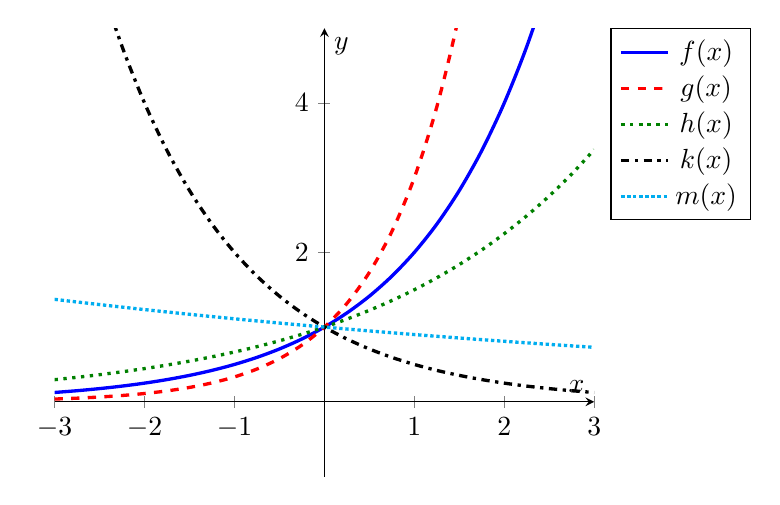
\begin{tikzpicture}
                \begin{axis}[axis lines=center, xlabel={$x$}, ylabel={$y$}, xmin=-3, xmax=3,
                    ymin=-1, ymax=5, domain=-3:3,legend pos=outer north east]
                    \addplot[smooth, blue, very thick] {2^x};
                    \addlegendentry{$f(x)$};
                    \addplot[smooth, red, very thick, dashed] {3^x};
                    \addlegendentry{$g(x)$};
                    \addplot[smooth, green!50!black, very thick, dotted] {1.5^x};
                    \addlegendentry{$h(x)$};
                    \addplot[smooth, black, very thick, dashdotted] {(0.5)^x};
                    \addlegendentry{$k(x)$};
                    \addplot[smooth, cyan, very thick, densely dotted] {(0.9)^x};
                    \addlegendentry{$m(x)$};
                \end{axis}
            \end{tikzpicture}
        \end{center}
        \caption{Exponential growth and decay functions} \label{F:0.2.Act1}
    \end{figure}
\end{activity}\aftera



\bex
One application to exponential decay is to calculate the intensity of radiation from
radioactive isotopes.  Most isotopes emit particles and decay into stable forms.  We
measure the rate of decay from the particles by the isotope's half-life, which is
how long it takes half of the isotope to decay.  The half-life for Sodium-25 ($Na^{25}$)
is almost exactly one minute.  Write a function that models that amount of $Na^{25}$ over
time if you start with exactly 36 grams.    
\eex
If you begin with 36 grams of $Na^{25}$ then the number of
grams remaining after $t$ minutes, $S(t)$, can be represented by the function
\[ S(t) = 36 \left( \frac{1}{2} \right)^{t}, \]
where $t$ is measured in minutes. Figure \ref{F:0.2.Ex1} shows this exponential decay
function with an initial value of 36 and a value of 18 after 1 day.
\begin{figure}[ht!]
    \begin{center}
%         \begin{tikzpicture}
%             \begin{axis}[axis lines=center, xlabel={$t$ (minutes)}, ylabel={$S(t)$
%                 (grams)}, xmin=0, xmax=5,ymin=0, ymax=40, domain=0:5]
%                 \addplot[blue, very thick, smooth] {36*(0.5)^x};
%                 \addplot[mark=*,red,very thick] coordinates{(1,18)};
%                 \addplot[mark=*,blue,very thick] coordinates{(0,36)};
%                 \draw (axis cs:1,18) node[anchor=west]{$(1,18)$};
%             \end{axis}
%         \end{tikzpicture}
        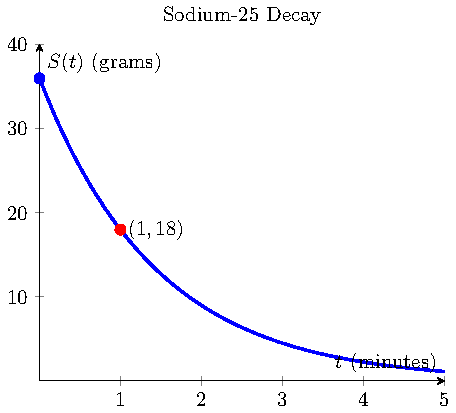
\includegraphics[width=0.5\columnwidth]{figures/0-2-fig2.pdf}
    \end{center}
    \caption{The grams of Sodium-25 remaining as a function of time. The blue point
    represents the initial value $(0,36)$ and the red point represents the value after 1
minute $(1,18)$.}
    \label{F:0.2.Ex1}
\end{figure}
\afterex

% \bigskip
\begin{activity}\label{A:0.2.2}
    A sample of $Ni^{56}$ has a half-life of 6.4 days.  Assume that there are 30 grams
    present initially.
    \ba
        \item Write a function describing the number of grams of $Ni^{56}$ present as a
            function of time.  Check your function based on the fact that in 6.4 days
            there should be 50\% remaining.
        \item What percent of the substance is present after 1 day?
        \item What percent of the substance is present after 10 days?
    \ea
\end{activity}
\begin{smallhint}
   \ba
        \item The growth rate should be $1/2$.
        \item Figure out how much is there after 1 day and divide by the original amount.
        \item Figure out how much is there after 10 days and divide by the original amount.
   \ea
\end{smallhint}
\begin{bighint}
   \ba
        \item When you substitute $6.4$ for the time you should have decayed by exactly
            half.
        \item Figure out how much is there after 1 day and divide by the original amount.
        \item Figure out how much is there after 10 days and divide by the original amount.
   \ea
\end{bighint}
\begin{activitySolution}
   \ba
        \item $A(t) = 30 \left( \frac{1}{2}  \right)^{t/6.4}$
        \item $A(1) =  30 \left( \frac{1}{2}  \right)^{1/6.4} \approx 26.9206$ so the
            percent that remains is just shy of 90\%.
        \item $A(10) =  30 \left( \frac{1}{2}  \right)^{10/6.4} \approx 10.1569$ so the
            percent that remains is about 33.9\%.
   \ea
\end{activitySolution}

\aftera


% \bigskip
\begin{activity}\label{A:0.2.3}\cite[p.9]{nonlinear}
    Uncontrolled geometric growth of the bacterium {\it Escherichia coli (E. Coli)} is the
    theme of the following quote taken from the best-selling author Michael Crichton's
    science fiction thriller, {\it The Andromeda Strain:}
    \begin{quote}
        ``The mathematics of uncontrolled growth are frightening.  A single cell of the
        bacterium E. coli would, under ideal circumstances, divide every twenty minutes.
        That is not particularly disturbing until you think about it, but the fact is that
        that bacteria multiply geometrically: one becomes two, two become four, four
        become eight, and so on.  In this way it can be shown that in a single day, one
        cell of E. coli could produce a super-colony equal in size and weight to the
        entire planet Earth.''
    \end{quote}
    \ba
        \item Write an equation for the number of E. coli cells present if a single cell
            of E. coli divides every 20 minutes. 
        \item How many E. coli would there be at the end of 24 hours?
        \item The mass of an E. coli bacterium is $1.7 \times 10^{-12}$ grams, while the
            mass of the Earth is $6.0 \times 10^{27}$ grams.  Is Michael Crichton's claim
            accurate?  Approximate the number of hours we should have allowed for this
            statement to be correct?
    \ea
\end{activity}\aftera


\subsection*{Investments}
Interest bearing bank accounts and investments follow exponential growth and decay models.
In the case of a savings account the interest is typically compounded several times per
year.  This means that the investor is getting interest on their interest every time the
bank computes the interest.    

% \begin{callout}
    If the money is gaining $p\%$ interest compounded $n$ times per year then the common ratio
for the exponential function is $1 + p/n$.  The exponent needs to reflect the fact that
the interest occurs at monthly intervals.  This means that the exponential function is
\begin{flalign}
    A(t) = A_0 \left( 1+\frac{p}{n} \right)^{nt} \quad \text{($t=$ number of years)}.
    \label{eqn:0.2.compound_interest}
\end{flalign}
In Equation \eqref{eqn:0.2.compound_interest}, $A_0$ is the initial investment, $A(t)$ is
the value of the investment over time, $p$ is the interest rate, and $n$ is the number of
times the interest is compounded per year.
% \end{callout}

\bex\label{0.2.Ex2}
If \$100 are invested into a bank account earning 2\% interest compounded 12 times per
year, how much does the investor have at the end of 1 year? 5 years? at retirement age?
How does this change is we compound quarterly or daily instead of monthly?
\eex
In the present situation the function modeling the value of the investment is
\[ A(t) = 100 \left( 1 + \frac{0.02}{12} \right)^{12t}. \]
Table \ref{tab:0.2.ex2} shows the value of the investment over the first 5 years.  It is
clear that this is very slow growth, but it is exponential none the less.  The common
ratio in this case is $r = (1+0.02/12) \approx 1.0017$, and this means that you are really
gaining 0.17\% interest per month.
\begin{table}[ht!]
    \centering
    \begin{tabular}{|c|c|c|c|c|c|c|}
        \hline
        Year & 0 & 1 & 2 & 3 & 4 & 5 \\ \hline
        Value & \$100 & \$102.02 & \$104.08 & \$106.18 & \$ 108.32 & \$ 110.51 \\ \hline
    \end{tabular}
    \caption{Value of \$100 investment for the first 5 years}
    \label{tab:0.2.ex2}
\end{table}

Assume that our investor was an 18 year old and extrapolate this to retirement age,
let's say 65 years old.  That is 47 years worth of interest, and the initial \$100
investment becomes 
\[ A(47) = 100 \left( 1 + \frac{0.02}{12} \right)^{12\cdot 47} \approx \$256. \]

If the number of times the bank compounds the interest changes the function will still
have essentially the same form: $A(t) = 100 (1+\frac{0.02}{n})^{nt}$. In Table
\ref{tab:0.2.ex2_n} the same investment is considered for several values of $n$.  While
more compoundings per year generally gives a higher rate of return on the investment, the
impact is small for larger values of $n$.  
\begin{table}[ht!]
    \centering
    \begin{tabular}{|c|c|c|c|c|c|c|c|c|}
        \hline
        Year & 0 & 1 & 2 & 3 & 4 & 5 & $\cdots$ & 47 \\ \hline
        Value ($n=1$) & \$100 & \$102.00 & \$104.04 & \$106.12 & \$ 108.24 & \$ 110.41 &
        $\cdots$ & \$253.63  \\ \hline
        Value ($n=4$) & \$100 & \$102.02 & \$104.07 & \$106.17 & \$ 108.31 & \$ 110.49 &
        $\cdots$ & \$255.40 \\ \hline
        Value ($n=12$) & \$100 & \$102.02 & \$104.08 & \$106.18 & \$ 108.32 & \$ 110.51 &
        $\cdots$ & \$255.80 \\ \hline
        Value ($n=365$) & \$100 & \$102.02 & \$104.08 & \$106.18 & \$ 108.33 & \$ 110.52 &
        $\cdots$ & \$255.99 \\ \hline
    \end{tabular}
    \caption{Value of \$100 investment for various values of $n$.}
    \label{tab:0.2.ex2_n}
\end{table}
\afterex

\subsection*{Exponential Functions with Base $e$}
Exponential functions are commonly written with a base of $e \approx 2.718281828459045\dots$.
This may seem like an arbitrary and bizarre choice at first glance, but we will see that this famous
number (called Euler's Number \footnote{Euler's number is named after the famous $17^{th}$
century mathematician Leonhard Euler. Euler was the first mathematician to introduce the
notion of a function, and he is responsible for a large amount of the development of
Calculus.}) plays a central role in Calculus.  

Euler's number can be derived from Equation \eqref{eqn:0.2.compound_interest} if we assume
that a fictitious bank gives $100\%$ interest compounded infinitely many times per year on
a one dollar investment.  Mathematically this is written as
\begin{flalign}
    e = 1 \cdot \left( 1 + \frac{1}{n} \right)^n \text{ as } n \to \infty.
    \label{eqn:0.2.euler}
\end{flalign}
\begin{table}[h!]
    \centering
    \begin{tabular}{|c|c|c|c|c|c|c|c|}
        \hline
        $n$ & $1$ & $10$ & $100$ & $1000$ & $\cdots$ & $10^{10}$& $\cdots$  \\ \hline
        $(1+\frac{1}{n})^n$ & $2$ & $2.5935$ & $2.7048$ & $2.7169$ & $\cdots$ & $2.71828$& $\cdots$  \\
        \hline
    \end{tabular}
    \caption{Approximations of Euler's number, $e$, using equation \eqref{eqn:0.2.euler} with various values of $n$}
    \label{tab:0.2.euler}
\end{table}

Any exponential function can be rewritten in terms of Euler's number in the form
\begin{flalign}
    f(x) = A e^{kx}.
    \label{eqn:0.2.exponential_e}
\end{flalign}
% \begin{callout}
In Equation \eqref{eqn:0.2.exponential_e}, $k$ is called the continuous
rate\index{continuous rate}.  
\begin{itemize}
    \item If $k>0$ then $f(x) = Ae^{kx}$ models exponential growth.
    \item If $k<0$ then $f(x) = Ae^{kx}$ models exponential decay.
\end{itemize}
% \end{callout}

\bex
A population of a city is 5000 people and is doubling in size every 5 years.  Use
equations \eqref{eqn:0.2.exponential} and \eqref{eqn:0.2.exponential_e} to write two
different functions modeling this population; one with base 2 and one with base $e$.
\eex
If the population is doubling every 5 years we can use equation
\eqref{eqn:0.2.exponential} to write
\[ P(t) = 5000 \cdot 2^{t/5}. \]
In order to use equation \eqref{eqn:0.2.exponential_e} we need to find the value of
``$k$''.  This is done by using the fact that at year 5 the population will be 10000 and
solving the equation
\[ 10000 = 5000 \cdot e^{5k}. \]
Rearranging we see that $e^{5k} = 2$.  In order to solve this algebraic equation we need
to use logarithms.  These important functions will be discussed in more detail in the
logarithms section %\ref{S:0.4.Logarithms}.  
In this case we see that $k = \ln(2) / 5 \approx 0.139.$
Therefore,
\[ P(t) = 5000 \cdot e^{0.139 t}. \]
Since these two equations model the same population they must be identical.  Indeed,
\[ 5000 \cdot 2^{t/5} = 5000 \cdot \left( 2^{1/5} \right)^t \approx 5000 \cdot (1.149)^t,
\]
and
\[ 5000 \cdot e^{kt} = 5000 \cdot \left( e^k \right)^t \approx 5000 \cdot (1.149)^t. \]
\afterex

% \begin{activity}\label{A:0.2.3}
The quantity, $Q$, of a drug in a patient's body at time $t$ is represented for positive
constants $S$ and $k$ by the function $Q(t) = S(1-e^{-kt})$. 
\ba
\item For $t \ge 0$ describe how $Q(t)$ changes with time.
\item Assuming that $S = 5$, use a graphing utility to make a sketch of $Q(t)$ with
    various values of $k$.  Use the left-hand side of Figure \ref{F:0.2.Act3} to organize
    your plots.  Interpret the value of $k$ in the context of this problem.
\item Now assume that $k=0.5$ and use a graphing utility to make a sketch of $Q(t)$ with
    various values of $S$.  Use the right-hand side of Figure \ref{F:0.2.Act3} to organize
    your plots.  Interpret the value of $S$ in the context of this problem.
\ea
\begin{figure}[h!]
    \begin{center}
        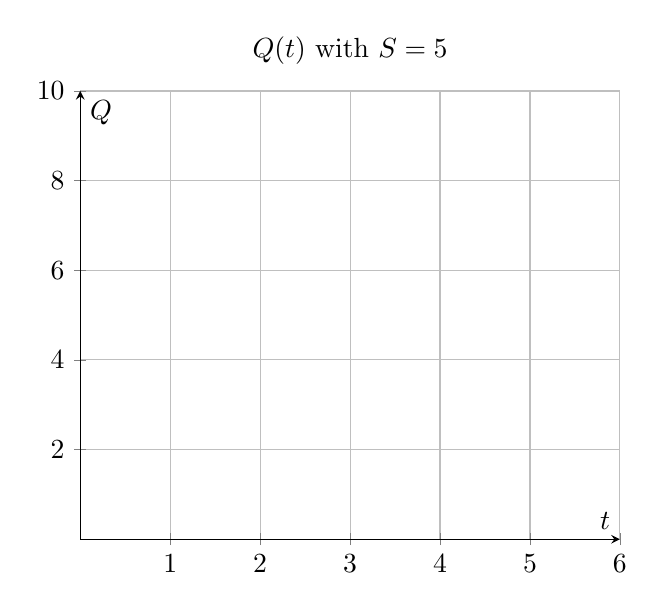
\begin{tikzpicture}
            \begin{axis}[axis lines=center,xlabel={$t$}, ylabel={$Q$}, xmin=0, ymin=0, xmax=6,
                ymax=10, grid, title={$Q(t)$ with $S=5$}]
                \addplot[smooth] {0*x};
            \end{axis}
        \end{tikzpicture}
        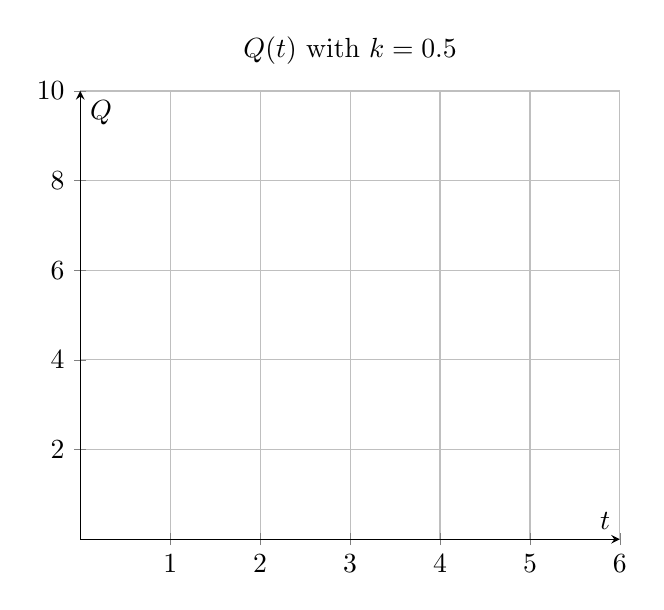
\begin{tikzpicture}
            \begin{axis}[axis lines=center,xlabel={$t$}, ylabel={$Q$}, xmin=0, ymin=0, xmax=6,
                ymax=10, grid, title={$Q(t)$ with $k=0.5$}]
                \addplot[smooth] {0*x};
            \end{axis}
        \end{tikzpicture}
    \end{center}
    \caption{Plot for Activity \ref{A:0.2.3}}
    \label{F:0.2.Act3}
\end{figure}
\end{activity}\aftera


% more activites

\begin{summary}
\item An exponential function can be written in the form $f(x) = A r^{kx}$ or $g(x) = A
    e^{kx}$.  
    \begin{itemize}
        \item In $f(x)$, if $k>0$ and $r>1$ then $f(x)$ models exponential growth.
        \item In $f(x)$, if $k>0$ and $0<r<1$ then $f(x)$ models exponential decay.
        \item In $g(x)$, if $k>0$ then $g(x)$ models exponential growth.
        \item In $g(x)$, if $k<0$ then $g(x)$ models exponential decay.
    \end{itemize}
\item Exponential functions have a constant common ratio for successive time values.
\end{summary}

\nin \hrulefill

% exercises go here
\begin{exercises} 

\item Suppose that $h(t) = A \cdot r^t$.  If $h(3)=4$ and $h(5)=40$,
    \ba
        \item find $r$.
        \item find $A$.
        \item Does this function model exponential growth or decay? How can you tell?
    \ea
\begin{exerciseSolution}
\end{exerciseSolution}


\item The half-life of $Br^{77}$ is 57 hours.
    \ba
        \item If the initial amount is $150$ grams, find the amount remaining after 171
            hours.
        \item Write an equation to predict the amount remaining after $t$ hours.
        \item Estimate within one hour how long it will take the amount to decrease to 10
            grams.
    \ea
\begin{exerciseSolution}
\end{exerciseSolution}


\item Consider the data in Table \ref{tab:0.2.exercise3}
    \ba
        \item Which (if any) of the functions could be linear? Explain how you know that
            these functions are linear, and find formulas for these functions.
        \item Which (if any) of the functions could be exponential? Explain how you know
            that these functions are linear, and find formulas for these functions.
    \ea
    \begin{table}[h!]
        \centering
        \begin{tabular}{|c|c|c|c|}
            \hline
            $x$ & $f(x)$ & $g(x)$ & $h(x)$ \\ \hline
           $-2$&$12$&$16$&$37$\\
           $-1$&$17$&$24$&$34$\\
           $0 $&$20$&$36$&$31$\\
           $1 $&$21$&$54$&$28$\\
           $2 $&$18$&$81$&$25$\\ \hline
        \end{tabular}
        \caption{Data tables for $f(x)$, $g(x)$, and $h(x)$}
        \label{tab:0.2.exercise3}
    \end{table}
\begin{exerciseSolution}
\end{exerciseSolution}

\end{exercises}
\afterexercises




\clearpage
